\documentclass[conference]{IEEEtran}
\IEEEoverridecommandlockouts
% The preceding line is only needed to identify funding in the first footnote. If that is unneeded, please comment it out.
\makeatletter
\def\endthebibliography{%
	\def\@noitemerr{\@latex@warning{Empty `thebibliography' environment}}%
	\endlist
}
\makeatother
\usepackage{cite}
\usepackage{amsmath,amssymb,amsfonts}
\usepackage{algorithmic}
\usepackage{hyperref}
\usepackage{graphicx}
\usepackage{textcomp}
\usepackage{xcolor}
\usepackage{adjustbox}
\usepackage{multirow}
\usepackage{subcaption}
\def\BibTeX{{\rm B\kern-.05em{\sc i\kern-.025em b}\kern-.08em
		T\kern-.1667em\lower.7ex\hbox{E}\kern-.125emX}}
\begin{document}
	
	\title{Multi-Modal Person Re-Identification using Lightweight Convolutional Neural Network}
	
	\makeatletter
	\newcommand{\linebreakand}{%
	\end{@IEEEauthorhalign}
	\hfill\mbox{}\par
	\mbox{}\hfill\begin{@IEEEauthorhalign}
	}
	\makeatother
	
	\author{
			\centering
		
		\IEEEauthorblockN{1\textsuperscript{st}Reza Fuad Rachmadi}
		\IEEEauthorblockA{\textit{Department of Computer Engineering} \\
			\textit{Faculty of Intelligent Electrical}\\
			\textit{and Informatics Technology}\\
			\textit{Institut Teknologi Sepuluh Nopember}\\
			Surabaya, Indonesia 60111 \\
			fuad@its.ac.id}
		\and
		\IEEEauthorblockN{2\textsuperscript{nd}I Ketut Eddy Purnama}
		\IEEEauthorblockA{\textit{Department of Computer Engineering} \\
			\textit{Faculty of Intelligent Electrical}\\
			\textit{and Informatics Technology}\\
			\textit{Institut Teknologi Sepuluh Nopember}\\
			Surabaya, Indonesia 60111 \\
			ketut@ee.its.ac.id}
		\and
		\IEEEauthorblockN{3\textsuperscript{rd} Charles Chang }
		\IEEEauthorblockA{\textit{Department of Computer Engineering} \\
			\textit{Faculty of Intelligent Electrical}\\
			\textit{and Informatics Technology}\\
			\textit{Institut Teknologi Sepuluh Nopember}\\
			Surabaya, Indonesia 60111 \\
			changcenliang@gmail.com}
		
	}

\maketitle

	
	
	\begin{abstract}
		\textit{As a complement to security systems, CCTVs are increasingly used to monitor and analyze criminal acts done at a given location. However, the manual search for criminals is still prone to human error. One of the solutions to make the process more effective and efficient is with the use of re-identification.
		Re-identification is a computer vision and deep learning technique in which an anonymized identity of an image is matched with its owner. In this paper, we will study the method of re-identifying people with multi-modal images where the query is in the form of a body sketch drawn by several different artists. The highest Rank-1 precision achieved in this paper with the Lightweight Convolutional Neural Network is 12\%.}
		
	\end{abstract}
	\begin{IEEEkeywords}
		\textit{CCTV, Re-Identification, Multi-modal, Criminal}
	\end{IEEEkeywords}
	
	\section{Introduction}
	\IEEEPARstart{O}{ver} the years, technology has improved and revolutionized our daily lives. More and more technology created to alleviate human life, such as CCTV cameras, are increasingly used to monitor public spaces. CCTV cameras have been a long-standing security measure used in public and commercial settings. The recordings from CCTV cameras provide vital visual information and can act as a witness to a crime scene. These recordings have a prominent role to play in providing evidence in criminal investigations and disputes.
	
	\vspace{1ex}
	
	According to data taken from the Central Bureau of Statistics, there is a rising crime wave throughout Indonesia. Polda Metro Jaya alone recorded the highest number of violations, namely 31,934 incidents\cite{cit:1, cit:2, cit:3, cit:4}. These facts encourage research on reducing the crime rate in various ways. Automation that can reduce the costs and workloads of the police force is needed. 
	
	\vspace{1ex}
	
	Person re-identification is a computer vision and deep learning technique in which an anonymized identity of a person is matched with its owner. Person re-identification can simplify many activities that were previously done manually, by establishing a person re-identification system, the inspection of recordings conducted by the police force can be carried out faster and can reduce the costs of labor.
	
	\vspace{1ex} 
	
	But a query photo of the target individual is not always readily available. Previous research of multi-modal person re-identification done by Lu Pang et al.\cite{cit:5} defined the problem of sketch re-identification, which uses a sketch instead of an image as the query of the model. While similar to facial sketch recognition, this problem is tackled using full-body sketches which add another dimension of complexity to the model. Furthermore, this problem is a challenging task due to the domain gap between sketch and photo. Sketches lack color information that is used as a differentiator between one individual and another. This study achieved Rank-1 precision of 34\% using a state-of-the-art model and cross-domain adversarial learning.
	
	\vspace{1ex} 
	
	In this paper, we investigated several lightweight Convolutional Neural Networks as a solution for sketch re-identification. We constructed the model based on the lightweight residual network used to solve the CIFAR dataset. We removed the fully connected layer of the original dataset and added two new fully connected layers.
	
	\section{Design and Implementation}
	\vspace{1ex}
	In this section, we will describe the design and implementation of lightweight Convolutional Neural Network for sketch re-identification. We will describe the experiment setting, the dataset used in the experiments, the training, and the testing processes.
	\vspace{1ex}
	\begin{figure}[!ht] \centering
		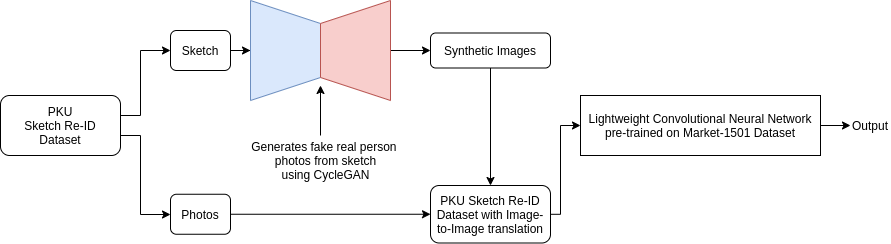
\includegraphics[width=0.5\textwidth]{img/desain_sistem.png}
		\caption{Block Diagram of Working System}
		\label{fig:1}
	\end{figure}
	
	\vspace{1ex}
	
	\subsection{Lightweight Convolutional Neural Network}
	\vspace{1ex}
	Figure 1 shows the diagram for our proposed lightweight Convolutional Neural Network classifier based on the architecture used to solve the CIFAR dataset. However, we removed the final fully connected layer and added two new ones at the end of the classifier to ensure the model learns good discriminatory features. Furthermore, unlike the original ResNet model, ours use an input resolution of 32x64x3 instead of 32x32x3. 
	
	In our experiments, we used two different lightweight residual networks, which are ResNet56 and ResNet110. Although the number of layers on these models is very deep, the number of parameters of the deepest classifier is still 1.7 million parameters which are less than the 23 million parameters that Resnet50 has.\\
	
	\begin{table}[h!]
		\begin{center}
			\begin{tabular}{|c|c|}
				\hline
				\textbf{Name} & \textbf{Parameters} \\ \hline
				ResNet56 & 0.85M \\ \hline
				ResNet110 & 1.7M \\ \hline
				GoogleNet & 7M \\ \hline
				DenseNet121 & 8.6M \\ \hline
				ResNet50 & 23M \\ \hline
			\end{tabular}
		\end{center}
		\vspace{1ex}
		\caption{Number of Parameters for Popular Models.}
		\label{tabel:1}
	\end{table}

	\subsection{PKU Sketch Re-ID Dataset}
	\vspace{1ex}
	
	\begin{figure}[h!] \centering
		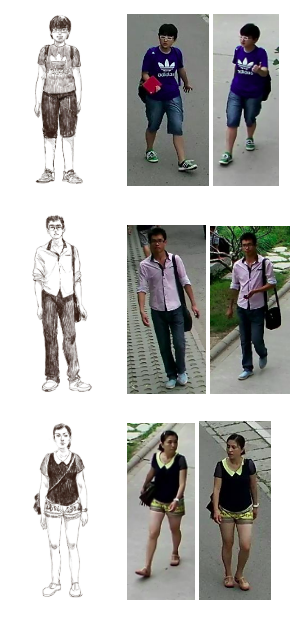
\includegraphics[width=0.25\textwidth]{img/ExamplesSketchReID.png}
		\caption{Examples of PKU Sketch ReID Data}
		\label{fig:2}
	\end{figure}
    
    \vspace{1ex}
	
	To evaluate the performance of our lightweight Convolutional Neural Network, we opted to use the PKU Sketch Re-ID dataset created by Lu Pang et al.. The dataset consists of 200 unique identities captured using two different cameras and one sketch corresponding to each individual, totaling 600 images. Figure 2 shows some examples of the dataset. The dataset was then divided into 150 identities for the training set and 50 identities for the testing set, as shown in figure 3. The images are manually cropped to ensure every photo contains one specific individual. As for the sketches, there are a total of five different artists to draw each identities sketches. Each artist has his/her own art style. 
	
	\begin{figure}[h!] \centering
		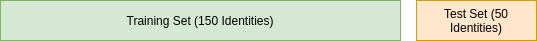
\includegraphics[width=0.48\textwidth]{img/TraintestSplit.png}
		\caption{Training-Testing Distribution}
		\label{fig:3}
	\end{figure}
	
	\vspace{1ex}
	
	\subsection{Cross Domain Image-to-Image Translation}
	\vspace{1ex}
	
	To help our model compensate for the lack of features in the query images, we decided to use image-to-image translation, specifically CycleGAN. CycleGAN allowed to mutually learn distributions of images, given two domains of the problems. GAN mimics the distribution of the generator given to the model which is photos and translates the style to generate synthetic photos from sketches. Essentially filling the gaps between the sketch and photos. Since the CycleGAN model is designed for unpaired translation, we created a paired testing set to ensure the style transfer is done between each unique individual. 
	
	For the CycleGAN, we used the model created by Jun-Yan Zhu et al. with the facades\_label2photo pre-trained weights. The images used to train the models are the 600 images from the PKU Sketch Re-ID. The model is trained for 200 epochs with the learning rate initialized at 0.0002 and decaying to 0.0001 after 150 epochs.
	
	\vspace{1ex}

	\subsection{Training and Testing Process}
	\vspace{1ex}
	
	\begin{figure}[h!] \centering
		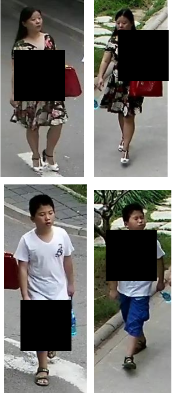
\includegraphics[width=0.15\textwidth]{img/RandomErasing.png}
		\caption{Examples of Random Erasing}
		\label{fig:4}
	\end{figure}
	
	To ensure the performance analysis is reliable, we perform the training and testing process ten times and take the average as the final evaluation metrics. All methods are evaluated using the Rank-1 accuracy of the model, following the baseline set by Lu Pang et al..
	
	\pagebreak
	
	In our experiments, we handled the lack of training data by pre-training on existing person re-id datasets. We used two different datasets which are the DukeMTMC and the Market-1501 dataset. The training process is done for 100 epochs with the learning rate initialized at 0.1. The learning rate is set to decay by a factor of 0.1 every 40 epochs. Furthermore, we used random erasing and random crop to add more training data. Figure 4 shows some examples of data augmentation using those two methods.
	
	\section{Results}
	\vspace{1ex}
	
	Based on the results of our experiments we decided to use a droprate of 0.5, a random erasing portion of 0.5, and only choose to continue with the ResNet56 and ResNet110 Convolutional Neural Network for further experimentation since it yields the best results. However, because a complete ablation study has not been done yet, the hyperparameters could still be tuned to increase the performance. 
	
	\begin{table}[h!]
		\begin{center}
			\begin{tabular}{|c|c|c|c|c|}
				\hline
				\textbf{Name} & \textbf{Rank-1} & \textbf{Rank-5} & \textbf{Rank-10} & \textbf{mAP} \\ \hline
				ResNet56 & 7.6\% & 27\% & 40.4\% & 10.46\%\\ \hline
				ResNet56 FC 1024 & 8.2\% & 29.2\% & 42.2\% & 10.99\%\\ \hline
				ResNet56 SPP & 8.4\% & 26.2\% & 40.2\% & 10.584\%\\ \hline
				ResNet110& 8.6\% & 29.6\% & 44.2\% & 10.95 \\ \hline
				ResNet110 FC 1024& 8.8\% & 29.6\% & 43.8\% & 11.3 \\ \hline
				ResNet110 SPP& 9.4\% & 25.6\% & 40.2\% & 11.254 \\ \hline
			\end{tabular}
		\end{center}
		\vspace{1ex}
		\caption{Summary of lightweight residual network classifier experiments on PKU Sketch Re-ID datasets (averaging from ten different runs).}
		\label{tabel:2}
	\end{table}
	
	To increase the performance of the classifier, we conducted an experiment making an ensemble from the tested ResNet56 and ResNet100 classifier. From the experiments conducted, the ensemble created could increase the performance of the model by 19\%, as seen on table III.
	
	\begin{table}[h!]
		\begin{center}
			\begin{tabular}{|c|c|c|c|c|}
				\hline
				\textbf{Name} & \textbf{Rank-1} & \textbf{Rank-5} & \textbf{Rank-10} & \textbf{mAP} \\ \hline
				Ensemble SPP & 10 \% & 26.2\% & 41.2\% & 10.46\%\\ \hline
				Ensemble FC 1024 & 10.2\% & 26.4\% & 41.4\% & 10.46\%\\ \hline
			\end{tabular}
		\end{center}
		\vspace{1ex}
		\caption{Experiments using Ensemble of ResNet56 and ResNet100 classifier (averaging from ten different runs).}
		\label{tabel:2}
	\end{table}
	
	\section{Comparison}
	\vspace{1ex}
	
	\begin{table}[h!]
		\begin{center}
			\begin{tabular}{|c|c|c|c|c|}
				\hline
				\textbf{Name} & \textbf{Parameters} & \textbf{Rank-1} & \textbf{Rank-5} & \textbf{Rank-10} \\ \hline
				Dense-HOG+LBP+rankSVM & ~8.6M & 5.1\% & 16.8\% & 28.3\% \\ \hline
				Triplet SN & n/a & 9\% & 26.8\% & 43.2\% \\ \hline
				GN Siamese & ~14M & 28.9\% & 54\% & 62.4\%\\ \hline
				Cross-Domain Adversarial & n/a & 34\% & 56.3\% & 72.5\%\\ \hline
				Ensemble SPP & ~3M& 10\% & 26.2\% & 41.2\% \\ \hline
				Ensemble FC 1024 & ~3M & 10.2\% & 26.4\% & 26.4 \%\\ \hline
			\end{tabular}
		\end{center}
		\vspace{1ex}
		\caption{Comparison to other state of the art models}
		\label{tabel:2}
	\end{table}
	
	
	Table IV shows the performance comparison of our model to several state-of-the-art models. Although the ensemble models does not have the best performance in Rank-5 and Rank-10 precision, we decided to evaluate all models using it's Rank-1 precision.
	
	\section{Conclusion}
	\vspace{1ex}
	In this paper, we introduce the usage of lightweight Convolutional Neural Network to tackle the problem of Sketch re-identification. To address the difference of modality in sketch and real images, we use image-to-image translation or more specifically CycleGAN. In the training process, we managed to have better precision compared to DenseNet, a classical model with more than quadruple the number of parameters that our model has. Other than that, or model prevailed against Triplet SN, a model composed of three identical Sketch-a-Nets and is optimized by triplet ranking loss. Although our model has not achieved state-of-the-art performance, the information gained by the classifier is very high, which proves the classifier is more efficient than other methods.
	
	\bibliographystyle{IEEEtran}
	\bibliography{dpustaka}
\end{document}
